\documentclass{article}[18pt]
\usepackage{../../../../../format}
\lhead{CSys - OS}


\begin{document}
\begin{center}
\underline{\huge Process Management}
\end{center}
\section{Process State}
As a process executes, it changes state:
\begin{itemize}
\item \textbf{New} - The process is being created
\item \textbf{Running} - Instructions are being executed
\item \textbf{Waiting} - The process is waiting for some event to occur
\item \textbf{Ready} - The process is ready to be dispatched to the CPU
\item \textbf{Terminated} - The process has completed its execution, or some other event causing termination
\end{itemize}
\section{Multiprogramming}
\textbf{Independent processes} cannot affect or be affected by the execution of other processes\\
\textbf{Co-operating processes} can affect or be affected by the execution of another process - there are advantages of implementing process co-operation\\
\\
The advantages of multiprogramming/implementing process co-operation may include::
\begin{itemize}
\item Computation speed-up: if there are multiple CPUs and/or cores
\item Convenience: single user wants to run many tasks
\item Information sharing: for example shared files
\item Modularity: programming (e.g. OOP)
\end{itemize}
Multiprogramming supports the co-operation of processes\\
\\
The aim of multiprogramming is to \textbf{maximise} CPU utilisation\\
\\
With multiprogramming several processes are kept in memory concurrently\\
\\
When one process is \textbf{waiting}, the operating system executes (to \textbf{running}) one of the processes sitting in the \textbf{ready} queue\\
\\
CPU scheduling is the method used to support multiprogramming in process management
\section{CPU Scheduling}
CPU scheduling can be viewed as processes 'taking turns'\\
\\
It provides a basis of fair and efficient sharing of system, in this case CPU, resources\\
\\
As the CPU is a primary computer resource therefore scheduling is fundamental to operating system design
\section{Schedulers}
An operating system operates three types of scheduler: long-term, medium, and short term
\begin{itemize}
\item The \textbf{long term scheduler(job scheduler)} selects which process should be brought into the ready queue
\item The \textbf{medium-term scheduler} removes processes from active contention for the CPU bv swapping processes in and out of the ready queue. This temporarily reduces the number of processes that the short-term scheduler (CPU scheduler must choose between)
\item The \textbf{short-term scheduler (CPU scheduler)} selects the process to be executed next and allocated to the CPU\\
\\
This decision is initiated when processes:
\begin{itemize}
\item Switch from running to waiting state
\item Switch from running to ready state
\item Switch from waiting to ready
\item Terminate
\end{itemize}
\end{itemize}
\subsection{Considerations}
Design considerations for scheduling.\\
\\
When the CPU switches to another process:
\begin{itemize}
\item The system must save the context of the old process
\item Load any saved context for the new process
\end{itemize}
Context-switch time is an \textbf{overhead}: the system undertakes no user processing while switching
\subsection{Criteria}
\begin{itemize}
\item CPU utilisation
\item Throughput: the number of processes that complete their execution within a specific number of time unit
\item Turnaround time: amount of time to execute a particular process
\item Waiting time: total (accumulated) amount of time a process has been waiting in the ready queue
\item Response time: amount of time it takes from when a request was first submitted to the ready queue until the first response is produced
\end{itemize}
\section{Scheduling Algorithms}
\subsection{Algorithm Evaluation}
\textbf{Deterministic modelling:}\\
Taking a predetermined workload (case) and analyse the performance of each algorithm\\
\\
\textbf{Simulation}:\\
Complex model of the system and the way it is used. Need to beware of Bonini's paradox\\
\\
\textbf{Post-implementation}:\\
Examine the running operating system
\subsection{Priority Scheduling}
In \textbf{priority scheduling}, the algorithm associates a priority number (integer for each process)\\
\\
The CPU is allocated by the dispatcher to the process with the highest priority\\
\\
\textbf{Problem:} Starvation - The low priority processes may never execute\\
\textbf{Solution:} Ageing - as time progresses increase the priority of the process\\
\\
Priority based CPU scheduling can be either pre-emptive or non pre emptive
\subsection{Multilevel queue scheduling}
Multilevel queue scheduling is where processes are partitioned into different queues, e.g. foreground vs background processes.\\
\\
The approach is based on the different queues having different (performance) requirements e.g. response time\\
\\
\textbf{Problem}: provides differentiation but not flexible, since a process remains in the same queue regardless of adapting requirements.\\
\textbf{Feedback queues}: An adaptation of multilevel queue scheduling, however the process may proceed from one queue to the next. This is the most common approach to scheduling but also difficult to implement.\\
\\
The \textbf{ready} queue is partitioned into separate queues\\
\\
Each queue has its own scheduling algorithm\\
\\
Scheduling must be undertaken between the queues
\begin{itemize}
\item Fixed priority scheduling
\item Time slice: each queue gets a certain amount of CPU time which it can schedule among its processes
\end{itemize}
\subsubsection{Multilevel feedback queue}
A process can move between the various queues\\
\\
A multilevel feedback queue scheduler may use the following parameters:
\begin{itemize}
\item The number of queues
\item The scheduling algorithms for each queue
\item The method used to determine when to upgrade a process
\item The method used to determine when to demote a process
\item The method used to determine which queue a process will enter
\end{itemize}


\subsection{First Come, First Served (FCFS)}
\begin{itemize}
\item The first process to request the CPU is allocated the CPU until it is completed
\end{itemize}
\begin{center}
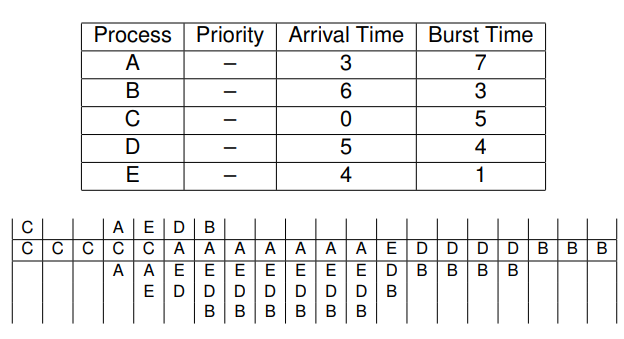
\includegraphics[scale=0.7]{FCFS}
\end{center}
\begin{itemize}
\item The average waiting time may or may not be lengthy
\item A simple algorithm to implement
\item May result in a 'convoy' effect, for example short processes waiting on a long process to finish
\end{itemize}
\subsection{Shortest-Job-First}
\begin{itemize}
\item Compares each process waiting to determine the length of its next CPU burst
\item Use these lengths to schedule the process with the shortest time (if two have the same length then FCFS)
\item Non pre emptive - once the CPU is given a process it cannot be pre-emptive until the process has completed its CPU Burst
\end{itemize}
\begin{center}
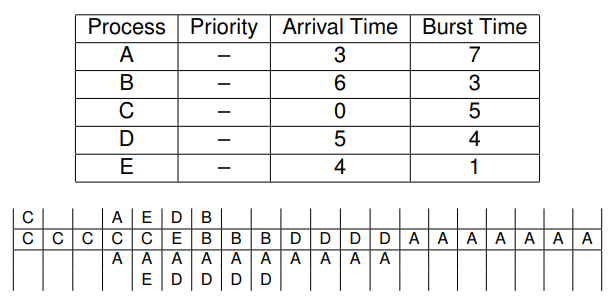
\includegraphics[scale=0.7]{SJF}
\end{center}
\subsection{Round Robin (RR)}
Each process gets a small unit of CPU time: a time quantum or time slice usually q=10 to 100 milliseconds\\
\\
After this time has elapsed, the process is pre-empted and added to the end of the ready queue\\
\\
If there are n processes in the ready queue and the time quantum is q, them each process gets $\frac{1}{n}$ of the CPU time in chunks of at most q time units at once
\begin{center}
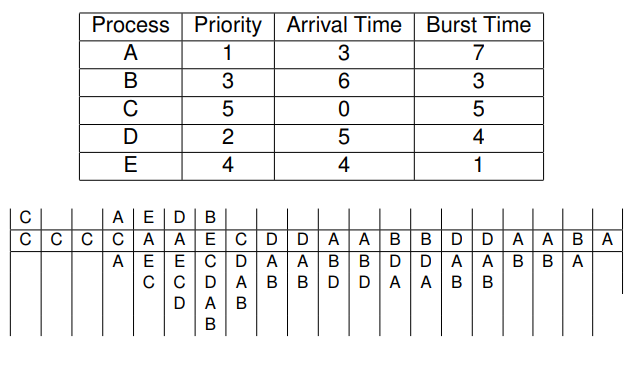
\includegraphics[scale=0.7]{RR}
\end{center}
\subsection{Shortest Remaining Time First}
If a new process arrives in the ready queue with a CPU burst length time less than the remaining time of the executing process then pre-empt the running process and run the process with the shorter CPU burst length.\\
\\
It can be viewed as a pre-emptive version of SJF.
\begin{center}
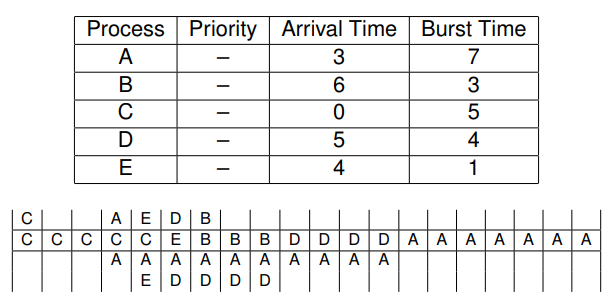
\includegraphics[scale=0.7]{SRTF1}
\end{center}
\begin{center}
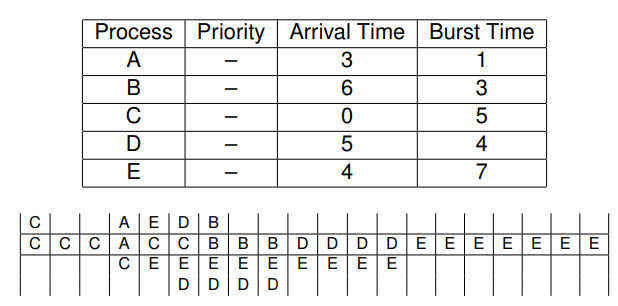
\includegraphics[scale=0.7]{SRTF2}
\end{center}
\subsection{Round Robin (With Priority)}
With priority in round robin, we can choose to implement either:
\begin{itemize}
\item a priority queue, or
\item a normal queue where the priority is used only when competing for entry onto the queue\\
\\
We will choose the latter
\end{itemize}
This is with time slice 2
\begin{center}
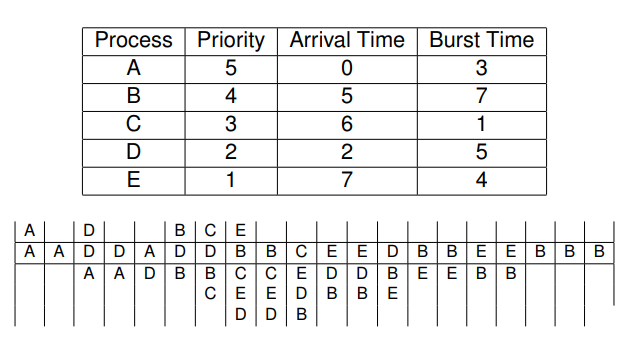
\includegraphics[scale=0.7]{RRP}
\end{center}

\end{document}